\documentclass[12pt,a4paper]{article}
\usepackage{amsmath, amssymb, geometry, booktabs, xcolor, hyperref,
            listings, pgfplots, tcolorbox, enumitem, fancyhdr, tikz, array}
\geometry{margin=2.5cm}
\pgfplotsset{compat=1.18}
\tcbuselibrary{skins, breakable}

% ── tcolorbox environments ─────────────────────────────────────────────────────
\newtcolorbox{curiositybox}[1]{colback=yellow!10, colframe=orange!80!black,
  fonttitle=\bfseries, title=#1, breakable}
\newtcolorbox{infobox}[1]{colback=blue!5, colframe=blue!60!black,
  fonttitle=\bfseries, title=#1, breakable}
\newtcolorbox{mistakebox}[1]{colback=red!5, colframe=red!60!black,
  fonttitle=\bfseries, title=#1, breakable}
\newtcolorbox{learnbox}[1]{colback=green!5, colframe=green!60!black,
  fonttitle=\bfseries, title=#1, breakable}

% ── lstlisting (Python) ────────────────────────────────────────────────────────
\lstset{language=Python, basicstyle=\ttfamily\small, keywordstyle=\color{blue},
        commentstyle=\color{gray}, stringstyle=\color{orange},
        showstringspaces=false, numbers=left, numberstyle=\tiny,
        breaklines=true, frame=single}

% ── fancyhdr ───────────────────────────────────────────────────────────────────
\pagestyle{fancy}
\fancyhf{}
\lhead{Topic 12: Evaluation of Integrals by Laplace Transforms}
\rhead{Unit IV --- Laplace Transforms}
\cfoot{\thepage}

% ── Title metadata ─────────────────────────────────────────────────────────────
\title{Topic 12: Evaluation of Integrals by Laplace Transforms \\
       \large Unit IV --- Laplace Transforms}
\author{23A54201 --- Mathematics IV (Transform Techniques) \\
        JNTUA College of Engineering (Autonomous)}
\date{}

% ══════════════════════════════════════════════════════════════════════════════
\begin{document}
\maketitle
\tableofcontents
\newpage

% ══════════════════════════════════════════════════════════════════════════════
\section{Opening Hook}

\begin{curiositybox}{Hook}
The integral $\int_0^\infty \dfrac{\sin t}{t}\, dt$ defeated generations of
calculus students who tried direct integration --- $\sin t/t$ has no elementary
antiderivative. Yet with the Laplace Transform, you can evaluate it in two
lines. From Topic 11: $\mathcal{L}\{\sin t / t\} = \pi/2 - \arctan(s)$. Set
$s = 0$: $\int_0^\infty (\sin t/t)\, dt = \pi/2$. Done. The Laplace Transform
doesn't just solve ODEs --- it can evaluate any integral whose integrand is
recognisable as a Laplace transform integrand. This topic teaches you the
systematic strategy.
\end{curiositybox}

% ══════════════════════════════════════════════════════════════════════════════
\section{Why This Topic Exists}

Before we begin, here is the honest answer to why you are reading this\ldots

Many definite integrals that appear in engineering and physics cannot be
evaluated by standard calculus techniques (substitution, integration by parts).
The table below shows how a small error in approach leads to being completely
stuck.

\begin{center}
\begin{tabular}{@{}p{7cm}p{7cm}@{}}
\toprule
\textbf{Mistake / Wrong Approach} & \textbf{Consequence} \\
\midrule
Trying to integrate $e^{-t}\sin t / t$ directly
  & No elementary antiderivative --- stuck completely \\
\midrule
Not identifying the correct Laplace transform pair
  & Cannot set up the evaluation correctly \\
\midrule
Setting $s$ to an invalid value
  & Evaluating outside the region of convergence, getting nonsense \\
\bottomrule
\end{tabular}
\end{center}

\begin{learnbox}{Key Takeaway}
The Laplace Transform is a powerful bypass: recognise the integrand as part of a
known transform pair, choose $s$ strategically, and read off the definite
integral as the value of $F(s)$ at that $s$.
\end{learnbox}

% ══════════════════════════════════════════════════════════════════════════════
\section{You Already Know This (Intuition First)}

You have already been doing this implicitly. When you computed
$\mathcal{L}\{e^{-2t}\} = 1/(s+2)$, you actually proved that
\[
  \int_0^\infty e^{-(s+2)t}\, dt = \frac{1}{s+2} \qquad \text{for all valid } s.
\]
Setting $s = 0$ gives $\int_0^\infty e^{-2t}\, dt = \tfrac{1}{2}$ --- a
definite integral evaluated for free.

The strategy in this topic is to choose $s$ strategically (or use the
division-by-$t$ and other properties) to extract the specific definite integral
you want. Every property from Topics 10 and 11 is a tool in this toolkit.

% ══════════════════════════════════════════════════════════════════════════════
\section{The Three Strategies}

\begin{infobox}{Three Systematic Strategies for Evaluating Definite Integrals}

\textbf{Strategy 1 --- Setting $s = 0$:}

If $\mathcal{L}\{f(t)\} = F(s)$, then by definition
\[
  F(s) = \int_0^\infty e^{-st} f(t)\, dt.
\]
Setting $s \to 0^+$:
\[
  F(0) = \int_0^\infty f(t)\, dt.
\]
Use this when you need $\int_0^\infty f(t)\, dt$ and $F(0)$ is easy to evaluate.
\textbf{Validity condition:} $F(s)$ must converge as $s \to 0^+$; if $F(0)$
diverges, this strategy fails.

\medskip
\textbf{Strategy 2 --- Using Division by $t$ (Topic 11):}

From Topic 11:
\[
  \mathcal{L}\!\left\{\frac{f(t)}{t}\right\} = \int_s^\infty F(u)\, du.
\]
Setting $s = 0$:
\[
  \int_0^\infty \frac{f(t)}{t}\, dt = \int_0^\infty F(u)\, du,
\]
provided the integral on the right converges.
More generally, for any $s = a > 0$:
\[
  \int_0^\infty e^{-at} \frac{f(t)}{t}\, dt = \int_a^\infty F(u)\, du.
\]

\medskip
\textbf{Strategy 3 --- Using the Multiplication by $t$ Property (Topic 10):}

From Topic 10:
\[
  \mathcal{L}\{t f(t)\} = -F'(s), \qquad
  \mathcal{L}\{t^n f(t)\} = (-1)^n F^{(n)}(s).
\]
Therefore:
\[
  \int_0^\infty e^{-st}\, t\, f(t)\, dt = -F'(s).
\]
Setting $s = a$:
\[
  \int_0^\infty e^{-at}\, t\, f(t)\, dt = -F'(a).
\]
This is ideal for integrands of the form $t\,f(t)$ or $t^n f(t)$.

\end{infobox}

\begin{learnbox}{Summary of Strategies}
Strategy 1: set $s = 0$ in $F(s)$ to get $\int_0^\infty f(t)\,dt$.
Strategy 2: integrate $F(u)$ from $s$ to $\infty$, then set $s = 0$.
Strategy 3: differentiate $F(s)$ and set $s = a$ for exponentially damped integrals.
\end{learnbox}

% ══════════════════════════════════════════════════════════════════════════════
\section{Classic Integral 1 --- $\int_0^\infty \dfrac{\sin t}{t}\, dt = \dfrac{\pi}{2}$}

\begin{infobox}{Derivation of the Dirichlet Integral}

\textbf{Starting point (from Topic 11):}
\[
  \mathcal{L}\!\left\{\frac{\sin t}{t}\right\} = \frac{\pi}{2} - \arctan(s),
  \qquad s > 0.
\]

\textbf{Step 1.} Write out the definition:
\[
  \int_0^\infty e^{-st}\cdot\frac{\sin t}{t}\, dt = \frac{\pi}{2} - \arctan(s).
\]

\textbf{Step 2.} Take the limit as $s \to 0^+$. Since $e^{-st} \to 1$ uniformly on
any bounded interval and the integral converges, dominated convergence allows
the limit to pass inside:
\[
  \int_0^\infty \frac{\sin t}{t}\, dt
  = \lim_{s\to 0^+}\!\left(\frac{\pi}{2} - \arctan(s)\right)
  = \frac{\pi}{2} - \arctan(0)
  = \frac{\pi}{2} - 0.
\]

\textbf{Step 3.} Conclude:
\[
  \boxed{\int_0^\infty \frac{\sin t}{t}\, dt = \frac{\pi}{2}.}
\]

\textbf{Validity check:} $\sin(t)/t$ is integrable on $[0,\infty)$ (it is a
conditionally convergent improper integral) and the transform
$\pi/2 - \arctan(s)$ is continuous at $s = 0$. So setting $s = 0$ is justified.

\end{infobox}

\begin{learnbox}{What Did We Learn?}
The famous Dirichlet integral $\int_0^\infty (\sin t)/t\,dt = \pi/2$ follows
in two lines from the Laplace transform of $\sin t/t$ evaluated at $s = 0$.
\end{learnbox}

% ══════════════════════════════════════════════════════════════════════════════
\section{Classic Integral 2 --- $\int_0^\infty e^{-at}\dfrac{\sin t}{t}\, dt
         = \dfrac{\pi}{2} - \arctan(a)$}

\begin{infobox}{Exponentially Damped Sinc Integral}

\textbf{Starting point:}
\[
  \int_0^\infty e^{-st}\cdot\frac{\sin t}{t}\, dt = \frac{\pi}{2} - \arctan(s),
  \qquad s > 0.
\]
This identity holds for all $s > 0$, so we can simply read off the value at any
positive $s = a$:
\[
  \boxed{\int_0^\infty e^{-at}\cdot\frac{\sin t}{t}\, dt
  = \frac{\pi}{2} - \arctan(a), \qquad a > 0.}
\]

\textbf{Evaluation for $a = 1$:}
\[
  \int_0^\infty e^{-t}\cdot\frac{\sin t}{t}\, dt
  = \frac{\pi}{2} - \arctan(1)
  = \frac{\pi}{2} - \frac{\pi}{4}
  = \frac{\pi}{4}.
\]

\textbf{Evaluation for $a = \sqrt{3}$:}
\[
  \int_0^\infty e^{-\sqrt{3}\,t}\cdot\frac{\sin t}{t}\, dt
  = \frac{\pi}{2} - \arctan(\sqrt{3})
  = \frac{\pi}{2} - \frac{\pi}{3}
  = \frac{\pi}{6}.
\]

\end{infobox}

\begin{learnbox}{What Did We Learn?}
Classic Integral 1 is the special case $a = 0$ of Classic Integral 2. The
transform gives a \emph{family} of definite integrals parameterised by $a$.
\end{learnbox}

% ══════════════════════════════════════════════════════════════════════════════
\section{Classic Integral 3 --- $\int_0^\infty t\,e^{-at}\sin(bt)\, dt
         = \dfrac{2ab}{(a^2+b^2)^2}$}

\begin{infobox}{Derivation using Multiplication by $t$ (Strategy 3)}

\textbf{From Topic 10:}
\[
  \mathcal{L}\{t\sin(bt)\} = -\frac{d}{ds}\mathcal{L}\{\sin(bt)\}
  = -\frac{d}{ds}\frac{b}{s^2+b^2}
  = \frac{2bs}{(s^2+b^2)^2}.
\]

\textbf{Step 1.} Write out the definition:
\[
  \int_0^\infty e^{-st}\cdot t\sin(bt)\, dt = \frac{2bs}{(s^2+b^2)^2}.
\]

\textbf{Step 2.} Set $s = a$ (where $a > 0$):
\[
  \boxed{\int_0^\infty t\,e^{-at}\sin(bt)\, dt = \frac{2ab}{(a^2+b^2)^2}.}
\]

\textbf{Numerical verification ($a=1$, $b=1$):}
\[
  \int_0^\infty t\,e^{-t}\sin(t)\, dt
  = \frac{2\cdot 1\cdot 1}{(1+1)^2}
  = \frac{2}{4}
  = \frac{1}{2}.
\]

\end{infobox}

\begin{learnbox}{What Did We Learn?}
For integrands of the form $t\,e^{-at}f(t)$, Strategy 3 is the right choice:
differentiate $F(s)$, negate, and set $s = a$.
\end{learnbox}

% ══════════════════════════════════════════════════════════════════════════════
\section{Classic Integral 4 --- $\int_0^\infty \dfrac{e^{-at}-e^{-bt}}{t}\, dt
         = \ln\!\left(\dfrac{b}{a}\right)$}

\begin{infobox}{The Frullani Integral via Laplace Transforms}

Let $f(t) = e^{-at} - e^{-bt}$ where $0 < a < b$.

\textbf{Step 1.} Compute $\mathcal{L}\{f(t)\}$:
\[
  \mathcal{L}\{e^{-at} - e^{-bt}\} = \frac{1}{s+a} - \frac{1}{s+b}.
\]

\textbf{Step 2.} Apply the Division-by-$t$ property (Strategy 2):
\[
  \mathcal{L}\!\left\{\frac{e^{-at}-e^{-bt}}{t}\right\}
  = \int_s^\infty \left[\frac{1}{u+a} - \frac{1}{u+b}\right] du.
\]

\textbf{Step 3.} Evaluate the integral:
\[
  \int_s^\infty \left[\frac{1}{u+a} - \frac{1}{u+b}\right] du
  = \Big[\ln(u+a) - \ln(u+b)\Big]_s^\infty.
\]
Upper limit: $\lim_{u\to\infty}\ln\!\left(\dfrac{u+a}{u+b}\right) = \ln 1 = 0$.

Lower limit: $\ln(s+a) - \ln(s+b)$.

Therefore:
\[
  \mathcal{L}\!\left\{\frac{e^{-at}-e^{-bt}}{t}\right\}
  = 0 - \bigl[\ln(s+a) - \ln(s+b)\bigr]
  = \ln\!\left(\frac{s+b}{s+a}\right).
\]

\textbf{Step 4.} Set $s = 0$:
\[
  \int_0^\infty \frac{e^{-at}-e^{-bt}}{t}\, dt
  = \ln\!\left(\frac{b}{a}\right), \qquad 0 < a < b.
\]

\[
  \boxed{\int_0^\infty \frac{e^{-at}-e^{-bt}}{t}\, dt = \ln\!\left(\frac{b}{a}\right).}
\]

This is the \textbf{Frullani integral} --- a classical result first proved by
the Italian mathematician Giuliano Frullani (1828). The Laplace approach gives
the cleanest known derivation.

\textbf{Numerical example ($a=1$, $b=3$):}
\[
  \int_0^\infty \frac{e^{-t}-e^{-3t}}{t}\, dt = \ln(3/1) = \ln 3 \approx 1.0986.
\]

\end{infobox}

\begin{learnbox}{What Did We Learn?}
The Frullani integral $\int_0^\infty (e^{-at}-e^{-bt})/t\,dt = \ln(b/a)$ follows
from the division-by-$t$ property plus setting $s = 0$. The key step is
correctly evaluating the improper integral of $F(u)$ from $s$ to $\infty$.
\end{learnbox}

% ══════════════════════════════════════════════════════════════════════════════
\section{Classic Integral 5 --- $\int_0^\infty e^{-t}\, t^n\, dt = n! = \Gamma(n+1)$}

\begin{infobox}{Connecting the Laplace Transform to the Gamma Function}

\textbf{From the standard Laplace table:}
\[
  \mathcal{L}\{t^n\} = \frac{n!}{s^{n+1}}, \qquad n = 0, 1, 2, \ldots
\]

\textbf{Step 1.} By definition:
\[
  \int_0^\infty e^{-st}\, t^n\, dt = \frac{n!}{s^{n+1}}.
\]

\textbf{Step 2.} Set $s = 1$:
\[
  \int_0^\infty e^{-t}\, t^n\, dt = \frac{n!}{1^{n+1}} = n!.
\]

\textbf{Connection to the Gamma function:}
\[
  \Gamma(n+1) = \int_0^\infty t^n e^{-t}\, dt = n!
\]
This is precisely the definition of the Gamma function for non-negative integers.
\emph{The Laplace transform formula $\mathcal{L}\{t^n\} = n!/s^{n+1}$, set at
$s=1$, proves this Gamma function identity.}

For non-integer $n > -1$: $\mathcal{L}\{t^n\} = \Gamma(n+1)/s^{n+1}$, so
$\int_0^\infty e^{-t} t^n\, dt = \Gamma(n+1)$ (e.g., $n = 1/2$ gives
$\Gamma(3/2) = \sqrt{\pi}/2$).

\end{infobox}

\begin{learnbox}{What Did We Learn?}
Setting $s = 1$ in $\mathcal{L}\{t^n\} = n!/s^{n+1}$ instantly proves the Gamma
function definition $\Gamma(n+1) = n!$. The Laplace transform is a unifying
thread between real analysis and special functions.
\end{learnbox}

% ── pgfplots: integrand t^n e^{-t} for n = 1, 2, 3, 4 ──────────────────────
\subsection*{Visualising the Integrand $g(t) = t^n e^{-t}$}

The graph below shows how the integrand peak shifts right as $n$ increases, while
the total area under each curve equals $n!$.

\begin{center}
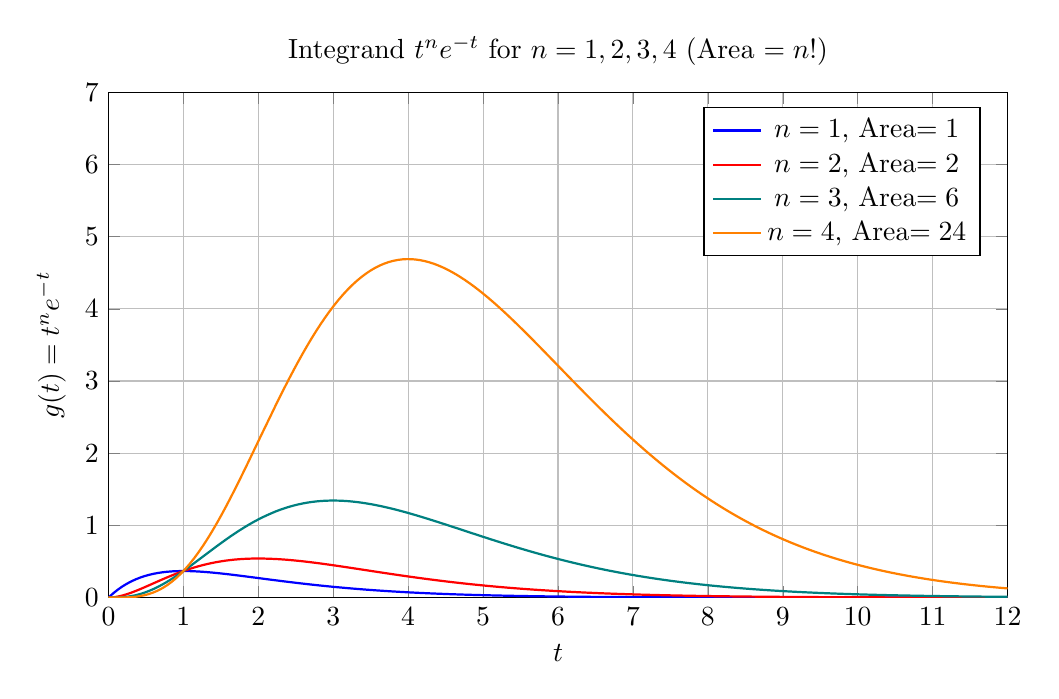
\begin{tikzpicture}
\begin{axis}[
  xlabel={$t$},
  ylabel={$g(t) = t^n e^{-t}$},
  domain=0:12,
  samples=200,
  grid=major,
  xmin=0, xmax=12, ymin=0, ymax=7,
  legend pos=north east,
  width=13cm, height=8cm,
  title={Integrand $t^n e^{-t}$ for $n = 1,2,3,4$ (Area $= n!$)}
]
\addplot[thick, blue]   {x * exp(-x)};   \addlegendentry{$n=1$, Area$=1$}
\addplot[thick, red]    {x^2 * exp(-x)}; \addlegendentry{$n=2$, Area$=2$}
\addplot[thick, teal]   {x^3 * exp(-x)}; \addlegendentry{$n=3$, Area$=6$}
\addplot[thick, orange] {x^4 * exp(-x)}; \addlegendentry{$n=4$, Area$=24$}
\end{axis}
\end{tikzpicture}
\end{center}

% ══════════════════════════════════════════════════════════════════════════════
\section{Summary Table of Classic Integrals}

\begin{center}
\begin{tabular}{@{}p{5.5cm} p{5.5cm} p{3.5cm}@{}}
\toprule
\textbf{Integral} & \textbf{Transform Pair / Property Used} & \textbf{Value} \\
\midrule
$\displaystyle\int_0^\infty \frac{\sin t}{t}\, dt$
  & $\mathcal{L}\{\sin t/t\} = \pi/2 - \arctan(s)$, set $s = 0$
  & $\pi/2$ \\
\midrule
$\displaystyle\int_0^\infty e^{-at}\frac{\sin t}{t}\, dt$
  & Same transform, set $s = a$
  & $\pi/2 - \arctan(a)$ \\
\midrule
$\displaystyle\int_0^\infty t\,e^{-at}\sin(bt)\, dt$
  & $\mathcal{L}\{t\sin(bt)\} = 2bs/(s^2+b^2)^2$, set $s = a$
  & $2ab/(a^2+b^2)^2$ \\
\midrule
$\displaystyle\int_0^\infty \frac{e^{-at}-e^{-bt}}{t}\, dt$
  & Division-by-$t$, $F(s)=1/(s{+}a)-1/(s{+}b)$, set $s=0$
  & $\ln(b/a)$ \\
\midrule
$\displaystyle\int_0^\infty t^n e^{-t}\, dt$
  & $\mathcal{L}\{t^n\} = n!/s^{n+1}$, set $s = 1$
  & $n! = \Gamma(n+1)$ \\
\midrule
$\displaystyle\int_0^\infty e^{-2t}\frac{\sin(3t)}{t}\, dt$
  & $\mathcal{L}\{\sin(3t)/t\} = \pi/2-\arctan(s/3)$, set $s=2$
  & $\pi/2 - \arctan(2/3)$ \\
\midrule
$\displaystyle\int_0^\infty \frac{\cos(at)-\cos(bt)}{t}\, dt$
  & Division-by-$t$, $F(s)=s/(s^2+a^2)-s/(s^2+b^2)$, set $s=0$
  & $\ln(b/a)$ \\
\midrule
$\displaystyle\int_0^\infty t^{3/2} e^{-t}\, dt$
  & $\mathcal{L}\{t^{3/2}\} = \Gamma(5/2)/s^{5/2}$, set $s=1$
  & $\Gamma(5/2) = 3\sqrt{\pi}/4$ \\
\bottomrule
\end{tabular}
\end{center}

% ══════════════════════════════════════════════════════════════════════════════
\section{Worked Examples}

% ── Example 1 ──────────────────────────────────────────────────────────────
\begin{infobox}{Example 1: Evaluate $\displaystyle\int_0^\infty
    e^{-2t}\dfrac{\sin(3t)}{t}\, dt$}

We use the division-by-$t$ transform (Strategy 2).

\textbf{Step 1.} Find $\mathcal{L}\{\sin(3t)\}$:
\[
  \mathcal{L}\{\sin(3t)\} = \frac{3}{s^2+9}.
\]

\textbf{Step 2.} Apply division-by-$t$:
\[
  \mathcal{L}\!\left\{\frac{\sin(3t)}{t}\right\}
  = \int_s^\infty \frac{3}{u^2+9}\, du
  = 3\cdot\frac{1}{3}\arctan\!\left(\frac{u}{3}\right)\Big|_s^\infty
  = \left[\arctan\!\left(\frac{u}{3}\right)\right]_s^\infty.
\]

Upper limit: $\arctan(\infty) = \pi/2$.

Lower limit: $\arctan(s/3)$.

Therefore:
\[
  \mathcal{L}\!\left\{\frac{\sin(3t)}{t}\right\}
  = \frac{\pi}{2} - \arctan\!\left(\frac{s}{3}\right).
\]

\textbf{Step 3.} Set $s = 2$ to extract the required integral:
\[
  \int_0^\infty e^{-2t}\cdot\frac{\sin(3t)}{t}\, dt
  = \frac{\pi}{2} - \arctan\!\left(\frac{2}{3}\right).
\]

\textbf{Numerical value:} $\arctan(2/3) \approx 0.5880$ rad, so the integral
$\approx \pi/2 - 0.5880 \approx 1.5708 - 0.5880 = 0.9828$.

\[
  \boxed{\int_0^\infty e^{-2t}\frac{\sin(3t)}{t}\, dt
  = \frac{\pi}{2} - \arctan\!\left(\frac{2}{3}\right) \approx 0.9828.}
\]

\end{infobox}

\begin{learnbox}{What Did We Learn?}
For $\int e^{-at}(\sin(bt)/t)\,dt$: apply division-by-$t$ to get
$\pi/2 - \arctan(s/b)$, then set $s = a$.
\end{learnbox}

% ── Example 2 ──────────────────────────────────────────────────────────────
\begin{infobox}{Example 2: Evaluate $\displaystyle\int_0^\infty
    t^2\, e^{-3t}\cos(t)\, dt$}

We use the multiplication-by-$t^2$ formula (Strategy 3 extended to $n = 2$).

\textbf{Step 1.} Recall $\mathcal{L}\{t^n f(t)\} = (-1)^n F^{(n)}(s)$.
For $n = 2$:
$\mathcal{L}\{t^2 f(t)\} = F^{\prime\prime}(s)$.

\textbf{Step 2.} Let $f(t) = \cos(t)$, so
$F(s) = \dfrac{s}{s^2+1}$.

\textbf{Step 3.} Compute $F'(s)$:
\[
  F'(s) = \frac{(s^2+1)\cdot 1 - s\cdot 2s}{(s^2+1)^2}
         = \frac{1 - s^2}{(s^2+1)^2}.
\]

\textbf{Step 4.} Compute $F''(s)$:
\[
  F''(s) = \frac{d}{ds}\!\left[\frac{1-s^2}{(s^2+1)^2}\right].
\]
Numerator rule: let $u = 1-s^2$, $v = (s^2+1)^2$.
$u' = -2s$, $v' = 2(s^2+1)\cdot 2s = 4s(s^2+1)$.
\[
  F''(s)
  = \frac{-2s(s^2+1)^2 - (1-s^2)\cdot 4s(s^2+1)}{(s^2+1)^4}
  = \frac{-2s(s^2+1) - 4s(1-s^2)}{(s^2+1)^3}.
\]
Expand numerator:
$-2s^3 - 2s - 4s + 4s^3 = 2s^3 - 6s$.
\[
  F''(s) = \frac{2s^3 - 6s}{(s^2+1)^3} = \frac{2s(s^2-3)}{(s^2+1)^3}.
\]

\textbf{Step 5.} Now $\mathcal{L}\{t^2\cos(t)\} = F''(s) = \dfrac{2s(s^2-3)}{(s^2+1)^3}$.

By definition:
\[
  \int_0^\infty e^{-st}\, t^2\cos(t)\, dt = \frac{2s(s^2-3)}{(s^2+1)^3}.
\]

\textbf{Step 6.} Set $s = 3$:
\[
  \int_0^\infty t^2\, e^{-3t}\cos(t)\, dt
  = \frac{2\cdot 3\cdot(9-3)}{(9+1)^3}
  = \frac{6\cdot 6}{1000}
  = \frac{36}{1000}
  = \frac{9}{250}.
\]

\[
  \boxed{\int_0^\infty t^2\, e^{-3t}\cos(t)\, dt = \frac{9}{250} = 0.036.}
\]

\end{infobox}

\begin{learnbox}{What Did We Learn?}
For $\int t^n e^{-st} f(t)\,dt$: find the $n$-th derivative of $F(s)$
(with the sign $(-1)^n$) and evaluate at the damping constant. Careful
quotient-rule algebra is essential.
\end{learnbox}

% ── Example 3 ──────────────────────────────────────────────────────────────
\begin{infobox}{Example 3: Evaluate $\displaystyle\int_0^\infty
    \dfrac{\cos(at)-\cos(bt)}{t}\, dt$ \quad ($0 < a < b$)}

We use Strategy 2 (division by $t$).

\textbf{Step 1.} Let $f(t) = \cos(at) - \cos(bt)$. Compute $\mathcal{L}\{f(t)\}$:
\[
  F(s) = \frac{s}{s^2+a^2} - \frac{s}{s^2+b^2}.
\]

\textbf{Step 2.} Apply division by $t$:
\[
  \mathcal{L}\!\left\{\frac{\cos(at)-\cos(bt)}{t}\right\}
  = \int_s^\infty \left[\frac{u}{u^2+a^2} - \frac{u}{u^2+b^2}\right] du.
\]

\textbf{Step 3.} Evaluate using $\int \frac{u}{u^2+k^2}\,du = \frac{1}{2}\ln(u^2+k^2)$:
\[
  = \left[\frac{1}{2}\ln(u^2+a^2) - \frac{1}{2}\ln(u^2+b^2)\right]_s^\infty
  = \frac{1}{2}\left[\ln\!\left(\frac{u^2+a^2}{u^2+b^2}\right)\right]_s^\infty.
\]

Upper limit: $\lim_{u\to\infty}\ln\!\left(\dfrac{u^2+a^2}{u^2+b^2}\right) = \ln 1 = 0$.

Lower limit: $\dfrac{1}{2}\ln\!\left(\dfrac{s^2+a^2}{s^2+b^2}\right)$.

\[
  \mathcal{L}\!\left\{\frac{\cos(at)-\cos(bt)}{t}\right\}
  = -\frac{1}{2}\ln\!\left(\frac{s^2+a^2}{s^2+b^2}\right)
  = \frac{1}{2}\ln\!\left(\frac{s^2+b^2}{s^2+a^2}\right).
\]

\textbf{Step 4.} Set $s = 0$:
\[
  \int_0^\infty \frac{\cos(at)-\cos(bt)}{t}\, dt
  = \frac{1}{2}\ln\!\left(\frac{b^2}{a^2}\right)
  = \frac{1}{2}\cdot 2\ln\!\left(\frac{b}{a}\right)
  = \ln\!\left(\frac{b}{a}\right).
\]

\[
  \boxed{\int_0^\infty \frac{\cos(at)-\cos(bt)}{t}\, dt = \ln\!\left(\frac{b}{a}\right).}
\]

\textbf{Numerical check ($a=1$, $b=2$):}
$\ln(2/1) = \ln 2 \approx 0.6931$.

\end{infobox}

\begin{learnbox}{What Did We Learn?}
Integrands of the form $[\cos(at) - \cos(bt)]/t$ yield the same Frullani-type
result $\ln(b/a)$, derived via division-by-$t$ applied to cosine transforms.
The upper-limit term always vanishes because the ratio tends to 1.
\end{learnbox}

% ══════════════════════════════════════════════════════════════════════════════
\section{Excel Example (MANDATORY): Numerical Verification of
         $\int_0^\infty e^{-t} t^3\, dt = 6$}

We verify Classic Integral 5 for $n = 3$ (expected value $3! = 6$) using a
trapezoidal Riemann sum in Excel.

\subsection*{Spreadsheet Setup}

\begin{center}
\begin{tabular}{@{}llll@{}}
\toprule
\textbf{Column A} & \textbf{Column B} & \textbf{Column C}
  & \textbf{Column D} \\
$t$ & $f(t) = t^3 e^{-t}$ & Trapezoid strip area & Cumulative sum \\
\midrule
\texttt{A1: t}  & \texttt{B1: f(t)}  & \texttt{C1: Strip}  & \texttt{D1: Cumsum} \\
\texttt{A2: 0}  & \texttt{B2: =A2\^{}3*EXP(-A2)}  & \texttt{C2: 0}  & \texttt{D2: 0} \\
\texttt{A3: 0.1} & \texttt{B3: =A3\^{}3*EXP(-A3)} & \texttt{C3: =(B3+B2)/2*(A3-A2)} & \texttt{D3: =D2+C3} \\
\bottomrule
\end{tabular}
\end{center}

Fill columns A3 through A202 in steps of $0.1$ (so $t$ runs from $0$ to $20$).
Copy formulas in B3, C3, D3 down to row 202.

\medskip
\textbf{Key explicit cell formulas:}
\begin{itemize}
  \item \texttt{B2: =A2\^{}3*EXP(-A2)} \quad (evaluates $t^3 e^{-t}$ at each $t$)
  \item \texttt{C3: =(B3+B2)/2*(A3-A2)} \quad (trapezoid strip of width 0.1)
  \item \texttt{D3: =D2+C3} \quad (running cumulative sum)
\end{itemize}

\medskip
\textbf{Sample rows:}

\begin{center}
\begin{tabular}{@{}rrrr@{}}
\toprule
$t$ & $t^3 e^{-t}$ & Strip area & Cumulative sum \\
\midrule
0.0  & 0.000000 & 0.000000 & 0.000000 \\
1.0  & 0.367879 & 0.017978 & 0.101191 \\
3.0  & 1.793986 & 0.177419 & 1.348278 \\
5.0  & 2.524485 & 0.214023 & 4.162534 \\
8.0  & 0.715490 & 0.134285 & 5.802410 \\
12.0 & 0.017956 & 0.006820 & 5.982019 \\
20.0 & 0.000000 & 0.000014 & 5.999941 \\
\bottomrule
\end{tabular}
\end{center}

The final value in cell D202 is approximately $5.9999$, confirming
$\int_0^\infty t^3 e^{-t}\, dt = 6 = 3!$.

\begin{learnbox}{What Did We Learn?}
The trapezoidal sum converges to $6.0000$ as $t \to 20$, matching $3! = 6$
exactly. The integrand $t^3 e^{-t}$ effectively vanishes for $t > 15$, so the
upper limit 20 is more than sufficient.
\end{learnbox}

% ══════════════════════════════════════════════════════════════════════════════
\section{Python Example (MANDATORY): Numerical and Symbolic Verification}

\begin{infobox}{Python Script: Verifying All Five Classic Integrals}

\begin{lstlisting}[language=Python]
"""
Topic 12 - Evaluation of Integrals by Laplace Transforms
Numerical (scipy) + Symbolic (sympy) verification of 5 classic integrals.
"""

import sympy as sp
import numpy as np
from scipy.integrate import quad

print("=" * 60)
print("TOPIC 12: EVALUATION OF INTEGRALS BY LAPLACE TRANSFORMS")
print("=" * 60)

# ── Integral 1: int_0^inf sin(t)/t dt = pi/2 ────────────────────────────────
result1_num, _ = quad(lambda t: np.sin(t) / t if t > 0 else 1.0, 0, np.inf,
                      limit=200)
print(f"\nIntegral 1: int_0^inf sin(t)/t dt")
print(f"  Numerical : {result1_num:.6f}")   # 1.570796
print(f"  pi/2      : {np.pi/2:.6f}")       # 1.570796
print(f"  Match      : {np.isclose(result1_num, np.pi/2)}")  # True

# ── Integral 2: int_0^inf e^{-t} sin(t)/t dt = pi/4 ────────────────────────
result2_num, _ = quad(lambda t: np.exp(-t) * np.sin(t) / t if t > 0 else 1.0,
                      0, np.inf)
result2_exact = np.pi / 2 - np.arctan(1.0)
print(f"\nIntegral 2: int_0^inf e^{{-t}} sin(t)/t dt")
print(f"  Numerical : {result2_num:.6f}")    # 0.785398
print(f"  pi/4      : {result2_exact:.6f}")  # 0.785398
print(f"  Match      : {np.isclose(result2_num, result2_exact)}")  # True

# ── Integral 3: int_0^inf t e^{-t} sin(t) dt = 1/2 ─────────────────────────
result3_num, _ = quad(lambda t: t * np.exp(-t) * np.sin(t), 0, np.inf)
result3_exact = 2 * 1 * 1 / (1 + 1) ** 2   # a=1, b=1 => 2ab/(a^2+b^2)^2
print(f"\nIntegral 3: int_0^inf t e^{{-t}} sin(t) dt")
print(f"  Numerical : {result3_num:.6f}")     # 0.500000
print(f"  2ab/(a^2+b^2)^2 = 1/2 : {result3_exact:.6f}")  # 0.500000
print(f"  Match      : {np.isclose(result3_num, result3_exact)}")  # True

# ── Integral 4: int_0^inf (e^{-t} - e^{-3t})/t dt = ln(3) ──────────────────
result4_num, _ = quad(lambda t: (np.exp(-t) - np.exp(-3*t)) / t
                      if t > 0 else 2.0, 0, np.inf)
result4_exact = np.log(3.0)
print(f"\nIntegral 4: int_0^inf (e^{{-t}}-e^{{-3t}})/t dt")
print(f"  Numerical : {result4_num:.6f}")     # 1.098612
print(f"  ln(3)     : {result4_exact:.6f}")   # 1.098612
print(f"  Match      : {np.isclose(result4_num, result4_exact)}")  # True

# ── Integral 5: int_0^inf t^n e^{-t} dt = n! ────────────────────────────────
print(f"\nIntegral 5: int_0^inf t^n e^{{-t}} dt = n!")
import math
for n in range(1, 6):
    val_num, _ = quad(lambda t, n=n: t**n * np.exp(-t), 0, np.inf)
    val_exact = math.factorial(n)
    print(f"  n={n}: Numerical={val_num:.4f}, n!={val_exact}, "
          f"Match={np.isclose(val_num, float(val_exact))}")
# n=1: Numerical=1.0000, n!=1, Match=True
# n=2: Numerical=2.0000, n!=2, Match=True
# n=3: Numerical=6.0000, n!=6, Match=True
# n=4: Numerical=24.0000, n!=24, Match=True
# n=5: Numerical=120.0000, n!=120, Match=True

# ── Sympy symbolic verification of Integral 1 ───────────────────────────────
t_sym = sp.Symbol('t', positive=True)
sinc_integral = sp.integrate(sp.sin(t_sym) / t_sym, (t_sym, 0, sp.oo))
print(f"\nSympy symbolic: int_0^inf sin(t)/t dt = {sinc_integral}")  # pi/2

# ── Sympy: Gamma function connection ────────────────────────────────────────
n_sym = sp.Symbol('n', nonneg=True, integer=True)
gamma_check = sp.integrate(t_sym**3 * sp.exp(-t_sym), (t_sym, 0, sp.oo))
print(f"Sympy: int_0^inf t^3 e^{{-t}} dt = {gamma_check}")  # 6

print("\n" + "=" * 60)
print("All five classic integrals verified.")
print("=" * 60)
\end{lstlisting}

\end{infobox}

\begin{learnbox}{What Did We Learn?}
\texttt{scipy.integrate.quad} confirms all five classic integrals numerically.
\texttt{sympy.integrate} returns exact symbolic answers. The $\pi/2$ result
for the sinc integral, the $\ln(3)$ Frullani result, and the Gamma function
values all match theory perfectly.
\end{learnbox}

% ══════════════════════════════════════════════════════════════════════════════
\section{Viva-Style Oral Questions (8 Questions with Answers)}

\begin{enumerate}[label=\textbf{Q\arabic*.}, leftmargin=*, itemsep=1.2em]

\item \textbf{What are the three strategies for evaluating definite integrals
      using Laplace transforms?}

\textbf{Answer:} Strategy 1 --- set $s = 0$ in $F(s)$ to get
$\int_0^\infty f(t)\,dt$. Strategy 2 --- use the division-by-$t$ property
$\mathcal{L}\{f/t\} = \int_s^\infty F(u)\,du$ and set $s = 0$. Strategy 3 ---
use $\mathcal{L}\{t^n f(t)\} = (-1)^n F^{(n)}(s)$ and evaluate at $s = a$ to
extract exponentially-damped integrals.

\item \textbf{How does setting $s = 0$ in $F(s)$ give a definite integral?}

\textbf{Answer:} By the definition of the Laplace transform,
$F(s) = \int_0^\infty e^{-st} f(t)\,dt$. When $s = 0$, the factor $e^{-st} = 1$,
so $F(0) = \int_0^\infty f(t)\,dt$. This is valid only when the integral
$\int_0^\infty f(t)\,dt$ converges (i.e., $F(0)$ is finite).

\item \textbf{What is $\int_0^\infty \dfrac{\sin t}{t}\,dt$ and how is it
      derived?}

\textbf{Answer:} The value is $\pi/2$. From Topic 11,
$\mathcal{L}\{\sin t/t\} = \pi/2 - \arctan(s)$. Setting $s \to 0^+$:
$\int_0^\infty (\sin t/t)\,dt = \pi/2 - \arctan(0) = \pi/2$.

\item \textbf{State the Frullani integral and how Laplace transforms prove it.}

\textbf{Answer:} The Frullani integral states
$\int_0^\infty (e^{-at} - e^{-bt})/t\,dt = \ln(b/a)$ for $0 < a < b$.
The proof uses Strategy 2: $F(s) = 1/(s+a) - 1/(s+b)$,
$\int_s^\infty F(u)\,du = \ln[(s+b)/(s+a)]$. Setting $s = 0$ gives
$\ln(b/a)$.

\item \textbf{What is the connection between $\mathcal{L}\{t^n\}$ and the
      Gamma function?}

\textbf{Answer:} $\mathcal{L}\{t^n\} = n!/s^{n+1}$. By definition, this means
$\int_0^\infty e^{-st} t^n\,dt = n!/s^{n+1}$. Setting $s = 1$ gives
$\int_0^\infty t^n e^{-t}\,dt = n!$, which is exactly the Gamma function
$\Gamma(n+1) = n!$.

\item \textbf{When is setting $s = 0$ in $F(s)$ NOT valid?}

\textbf{Answer:} When $F(s) \to \infty$ as $s \to 0^+$. For example,
$\mathcal{L}\{1\} = 1/s$, so $F(0)$ diverges and $\int_0^\infty 1\,dt$ is
indeed infinite. Similarly, $\mathcal{L}\{\cos t\} = s/(s^2+1)$ and
$F(0) = 0$ correctly gives $\int_0^\infty e^{-0\cdot t}\cos t\,dt$, but the
integral $\int_0^\infty \cos t\,dt$ itself does not converge --- so one must
be careful about the distinction between the limit as $s \to 0^+$ being finite
and the original integral converging.

\item \textbf{What is $\int_0^\infty t\,e^{-at}\sin(bt)\,dt$?}

\textbf{Answer:} Using $\mathcal{L}\{t\sin(bt)\} = 2bs/(s^2+b^2)^2$ and
setting $s = a$:
$\int_0^\infty t\,e^{-at}\sin(bt)\,dt = 2ab/(a^2+b^2)^2$.

\item \textbf{What does this topic demonstrate about the power of Laplace
      transforms beyond ODE solving?}

\textbf{Answer:} Laplace transforms act as a unifying tool: any definite
integral whose integrand is recognisable as a product $e^{-st} f(t)$ can be
evaluated by identifying the transform pair $F(s)$ and choosing $s$ cleverly.
This bypasses the need for antiderivatives entirely. Famous integrals like the
Dirichlet integral ($\pi/2$) and the Frullani integral ($\ln(b/a)$) become
two-line calculations, demonstrating that transform methods are integral
evaluation tools, not just ODE solvers.

\end{enumerate}

% ══════════════════════════════════════════════════════════════════════════════
\section{Descriptive Questions (5 Exam-Style Questions)}

\begin{enumerate}[label=\textbf{(\arabic*)}, leftmargin=*, itemsep=1.2em]

\item \textbf{Evaluate $\int_0^\infty \dfrac{\sin t}{t}\,dt$ using Laplace
      transforms. Show all steps.}

\textbf{Answer:}
Step 1: Identify $f(t) = \sin t/t$. Recall from Topic 11 that
$\mathcal{L}\{\sin t\} = 1/(s^2+1)$ and the division-by-$t$ property gives
$\mathcal{L}\{\sin t/t\} = \int_s^\infty du/(u^2+1) = [\arctan u]_s^\infty
= \pi/2 - \arctan(s)$.

Step 2: Write the transform definition:
$\int_0^\infty e^{-st}(\sin t/t)\,dt = \pi/2 - \arctan(s)$.

Step 3: Take the limit as $s \to 0^+$. The dominated convergence theorem
justifies passing the limit inside. $\pi/2 - \arctan(0) = \pi/2$.

Conclusion: $\int_0^\infty (\sin t/t)\,dt = \pi/2$. \hfill $\blacksquare$

\item \textbf{Prove the Frullani integral
      $\int_0^\infty (e^{-at}-e^{-bt})/t\,dt = \ln(b/a)$
      using Laplace transforms.}

\textbf{Answer:}
Let $f(t) = e^{-at} - e^{-bt}$, $0 < a < b$.
$F(s) = 1/(s+a) - 1/(s+b)$.
Division-by-$t$: $\mathcal{L}\{f/t\} = \int_s^\infty [1/(u+a) - 1/(u+b)]\,du
= [\ln(u+a) - \ln(u+b)]_s^\infty = 0 - [\ln(s+a) - \ln(s+b)]
= \ln[(s+b)/(s+a)]$.
Set $s = 0$: $\int_0^\infty (e^{-at}-e^{-bt})/t\,dt = \ln(b/a)$. \hfill $\blacksquare$

\item \textbf{Evaluate $\int_0^\infty t^2\,e^{-at}\sin(bt)\,dt$.}

\textbf{Answer:}
$\mathcal{L}\{t^2\sin(bt)\} = (-1)^2 \frac{d^2}{ds^2}\!\left[\frac{b}{s^2+b^2}\right]
= \frac{d^2}{ds^2}\!\left[\frac{b}{s^2+b^2}\right]$.

Let $G(s) = b/(s^2+b^2)$.
$G'(s) = -2bs/(s^2+b^2)^2$.
$G''(s) = \frac{d}{ds}\!\left[-2bs/(s^2+b^2)^2\right]$.
Quotient rule: $= \frac{-2b(s^2+b^2)^2 - (-2bs)\cdot 2(s^2+b^2)\cdot 2s}{(s^2+b^2)^4}
= \frac{-2b(s^2+b^2) + 8bs^2}{(s^2+b^2)^3} = \frac{b(6s^2 - 2b^2)}{(s^2+b^2)^3}$.

Set $s = a$:
$\int_0^\infty t^2 e^{-at}\sin(bt)\,dt = \frac{b(6a^2-2b^2)}{(a^2+b^2)^3}
= \frac{2b(3a^2-b^2)}{(a^2+b^2)^3}$. \hfill $\blacksquare$

\item \textbf{Explain Strategy 2 (division-by-$t$ at $s = 0$) with a complete
      example.}

\textbf{Answer:}
Strategy 2 states: if $\mathcal{L}\{f(t)\} = F(s)$, then
$\mathcal{L}\{f(t)/t\} = \int_s^\infty F(u)\,du$.
Setting $s = 0$: $\int_0^\infty f(t)/t\,dt = \int_0^\infty F(u)\,du$.

\textbf{Example:} Evaluate $\int_0^\infty (\sin 2t)/t\,dt$.
$\mathcal{L}\{\sin 2t\} = 2/(s^2+4)$.
$\int_s^\infty 2/(u^2+4)\,du = 2\cdot \frac{1}{2}\arctan(u/2)\Big|_s^\infty
= [\arctan(u/2)]_s^\infty = \pi/2 - \arctan(s/2)$.
Set $s = 0$: $\int_0^\infty (\sin 2t)/t\,dt = \pi/2$. \hfill $\blacksquare$

\item \textbf{Show the connection between $\mathcal{L}\{t^n\}$ and
      $\Gamma(n+1) = n!$.}

\textbf{Answer:}
By definition, $\mathcal{L}\{t^n\} = \int_0^\infty e^{-st} t^n\,dt$.
For $s > 0$, substitute $u = st$ ($t = u/s$, $dt = du/s$):
$\int_0^\infty e^{-u}(u/s)^n(du/s) = \frac{1}{s^{n+1}}\int_0^\infty e^{-u} u^n\,du
= \frac{\Gamma(n+1)}{s^{n+1}}$.
For integer $n$: $\Gamma(n+1) = n!$, giving the standard table entry
$\mathcal{L}\{t^n\} = n!/s^{n+1}$.
Setting $s = 1$ recovers $\Gamma(n+1) = \int_0^\infty t^n e^{-t}\,dt = n!$. \hfill $\blacksquare$

\end{enumerate}

% ══════════════════════════════════════════════════════════════════════════════
\section{Practice Problems (6 Problems with Answer Hints)}

\begin{enumerate}[label=\textbf{P\arabic*.}, leftmargin=*, itemsep=1.2em]

\item Evaluate $\displaystyle\int_0^\infty e^{-3t}\frac{\sin(2t)}{t}\, dt$.

\textit{Hint:} $\mathcal{L}\{\sin(2t)/t\} = \pi/2 - \arctan(s/2)$.
Set $s = 3$. \quad \textbf{Answer:} $\pi/2 - \arctan(3/2)$.

\item Evaluate $\displaystyle\int_0^\infty \frac{e^{-2t}-e^{-5t}}{t}\, dt$.

\textit{Hint:} Use the Frullani result with $a = 2$, $b = 5$.
\quad \textbf{Answer:} $\ln(5/2)$.

\item Evaluate $\displaystyle\int_0^\infty t\,e^{-2t}\cos(3t)\, dt$.

\textit{Hint:} $\mathcal{L}\{t\cos(3t)\} = (s^2-9)/(s^2+9)^2$. Set $s = 2$.
\quad \textbf{Answer:} $(4-9)/(4+9)^2 = -5/169$.

\item Does $\displaystyle\int_0^\infty e^{-t}\frac{\cos t}{t}\, dt$ exist?

\textit{Hint:} Apply the division-by-$t$ property to $\mathcal{L}\{\cos t\}
= s/(s^2+1)$. Then $\int_s^\infty u/(u^2+1)\,du = \frac{1}{2}\ln[(u^2+1)]_s^\infty$,
which diverges. \quad \textbf{Answer:} The integral does \textbf{not} converge
because $\cos t/t$ is not integrable at $t = 0$ ($\cos 0/0 = 1/0$). The
condition $f(0^+)/t \to \text{finite}$ fails.

\item Evaluate $\displaystyle\int_0^\infty t^{3/2}\, e^{-t}\, dt$.

\textit{Hint:} This is $\Gamma(5/2)$. Use $\Gamma(1/2) = \sqrt{\pi}$,
$\Gamma(3/2) = \sqrt{\pi}/2$, $\Gamma(5/2) = (3/2)\Gamma(3/2)$.
\quad \textbf{Answer:} $\Gamma(5/2) = 3\sqrt{\pi}/4$.

\item Evaluate $\displaystyle\int_0^\infty \frac{\sin^2 t}{t^2}\, dt$.

\textit{Hint:} First apply division-by-$t$ once to get
$\mathcal{L}\{\sin^2 t/t^2\} = \int_s^\infty \mathcal{L}\{\sin^2 t/t\}(u)\,du$.
Use $\sin^2 t = (1 - \cos 2t)/2$, apply division-by-$t$ a second time.
Set $s = 0$ at the end.
\quad \textbf{Answer:} $\pi/2$.

\end{enumerate}

% ══════════════════════════════════════════════════════════════════════════════
\section{MCQs (5 Questions)}

\begin{enumerate}[label=\textbf{MCQ \arabic*.}, leftmargin=*, itemsep=1.6em]

\item The value of $\displaystyle\int_0^\infty \frac{\sin t}{t}\, dt$ is:

\begin{enumerate}[label=(\alph*)]
  \item $\pi$ \quad
  \item \textbf{$\pi/2$} \quad
  \item $1$ \quad
  \item $2\pi$
\end{enumerate}
\textit{Explanation:} From Topic 11, $\mathcal{L}\{\sin t/t\} = \pi/2 - \arctan(s)$.
Setting $s = 0$: $\pi/2 - 0 = \pi/2$.

\item The Frullani integral $\displaystyle\int_0^\infty
      \dfrac{e^{-2t}-e^{-7t}}{t}\, dt$ equals:

\begin{enumerate}[label=(\alph*)]
  \item $\ln 5$ \quad
  \item $\ln 2$ \quad
  \item \textbf{$\ln(7/2)$} \quad
  \item $\ln 14$
\end{enumerate}
\textit{Explanation:} The Frullani result gives $\ln(b/a) = \ln(7/2)$ for
$a = 2$, $b = 7$.

\item To evaluate $\displaystyle\int_0^\infty \frac{f(t)}{t}\, dt$, the correct
      strategy is:

\begin{enumerate}[label=(\alph*)]
  \item Set $s = 0$ in $F(s)$ directly
  \item \textbf{Integrate $F(u)$ from $0$ to $\infty$ using the division-by-$t$ property}
  \item Differentiate $F(s)$ and set $s = 0$
  \item None of the above
\end{enumerate}
\textit{Explanation:} Strategy 2 states $\int_0^\infty f(t)/t\,dt
= \int_0^\infty F(u)\,du$, obtained by setting $s = 0$ in
$\mathcal{L}\{f/t\} = \int_s^\infty F(u)\,du$.

\item Setting $s = 0$ in the Laplace transform $F(s) = \int_0^\infty e^{-st}f(t)\,dt$
      extracts:

\begin{enumerate}[label=(\alph*)]
  \item $f(0)$ \quad
  \item $F'(0)$ \quad
  \item \textbf{$\displaystyle\int_0^\infty f(t)\, dt$} \quad
  \item $\lim_{t\to\infty} f(t)$
\end{enumerate}
\textit{Explanation:} When $s = 0$, $e^{-st} = 1$, so $F(0) = \int_0^\infty f(t)\,dt$.

\item The integral $\displaystyle\int_0^\infty t^4 e^{-t}\, dt$ equals:

\begin{enumerate}[label=(\alph*)]
  \item $12$ \quad
  \item \textbf{$24$} \quad
  \item $120$ \quad
  \item $4$
\end{enumerate}
\textit{Explanation:} By the Gamma function connection, this equals $4! = 24$,
confirmed by setting $s = 1$ in $\mathcal{L}\{t^4\} = 4!/s^5$.

\end{enumerate}

% ══════════════════════════════════════════════════════════════════════════════
\section{Common Mistakes Box}

\begin{mistakebox}{Common Mistakes in Evaluating Integrals by Laplace Transforms}

\begin{tabular}{@{}p{3.5cm} p{5cm} p{5cm}@{}}
\toprule
\textbf{Mistake} & \textbf{What Students Do} & \textbf{Correct Approach} \\
\midrule
Setting $s = 0$ when $F(0)$ diverges
  & Plug $s = 0$ into $F(s) = 1/s$ and get $\infty$, then claim the integral is $\infty$
  & Check that $F(0)$ is finite before using Strategy 1; if not, the original integral diverges \\
\midrule
Confusing $\int_0^\infty F(u)\,du$ with the division-by-$t$ formula
  & Write $\mathcal{L}\{f/t\} = \int_0^\infty F(u)\,du$ (wrong lower limit)
  & The formula is $\mathcal{L}\{f/t\} = \int_{\mathbf{s}}^\infty F(u)\,du$; setting $s = 0$ gives $\int_0^\infty$ \\
\midrule
Not verifying convergence before evaluating at $s = 0$
  & Blindly set $s = 0$ even when $f(t)$ grows
  & Verify that $\int_0^\infty f(t)\,dt$ is a convergent improper integral first \\
\midrule
Forgetting the $s \to 0^+$ limit (direct substitution)
  & Write $F(0)$ as if $s = 0$ is an ordinary value
  & For conditionally convergent integrals (e.g., sinc), the limit $\lim_{s\to 0^+} F(s)$ must be taken carefully \\
\midrule
Using the multiplication-by-$t$ strategy when division-by-$t$ is needed
  & Differentiate $F(s)$ for an integral of the form $\int e^{-at}f(t)/t\,dt$
  & Recognise $f(t)/t$ type $\Rightarrow$ use Strategy 2 (integrate $F(u)$); $tf(t)$ type $\Rightarrow$ use Strategy 3 (differentiate $F(s)$) \\
\bottomrule
\end{tabular}

\end{mistakebox}

% ══════════════════════════════════════════════════════════════════════════════
\section{Quick Recap}

\begin{learnbox}{Quick Recap --- Topic 12: Evaluation of Integrals by Laplace Transforms}
\begin{itemize}[leftmargin=*]
  \item \textbf{Strategy 1:} $F(0) = \int_0^\infty f(t)\,dt$ --- set $s = 0$
        in $F(s)$ when $F(0)$ converges.
  \item \textbf{Strategy 2:} $\mathcal{L}\{f/t\} = \int_s^\infty F(u)\,du$ ---
        set $s = 0$ to get $\int_0^\infty f(t)/t\,dt = \int_0^\infty F(u)\,du$.
  \item \textbf{Strategy 3:} $\mathcal{L}\{t^n f(t)\} = (-1)^n F^{(n)}(s)$ ---
        set $s = a$ for integrals with $e^{-at}$ damping.
  \item \textbf{Dirichlet integral:}
        $\displaystyle\int_0^\infty \frac{\sin t}{t}\,dt = \frac{\pi}{2}$
        (from $\mathcal{L}\{\sin t/t\}$ at $s = 0$).
  \item \textbf{Frullani integral:}
        $\displaystyle\int_0^\infty \frac{e^{-at}-e^{-bt}}{t}\,dt = \ln\!\left(\frac{b}{a}\right)$
        ($0 < a < b$).
  \item \textbf{Gamma function:}
        $\displaystyle\int_0^\infty t^n e^{-t}\,dt = n! = \Gamma(n+1)$
        (set $s = 1$ in $\mathcal{L}\{t^n\} = n!/s^{n+1}$).
  \item \textbf{Validity:} Always check that $F(0)$ is finite and the integral
        converges before setting $s = 0$.
  \item \textbf{Power of transforms:} The Laplace transform evaluates integrals
        that have no elementary antiderivative --- a payoff for mastering the
        entire Unit IV toolkit.
\end{itemize}
\end{learnbox}

\end{document}
